% Selected real-scene visualization and current Table 1 Native results, 2026-11-04.
% \begin{center}
% \captionsetup{type=figure}
% % Match the 2260:40:1350 widths of the previous 3650-unit canvas.
\makebox[\textwidth]{%
  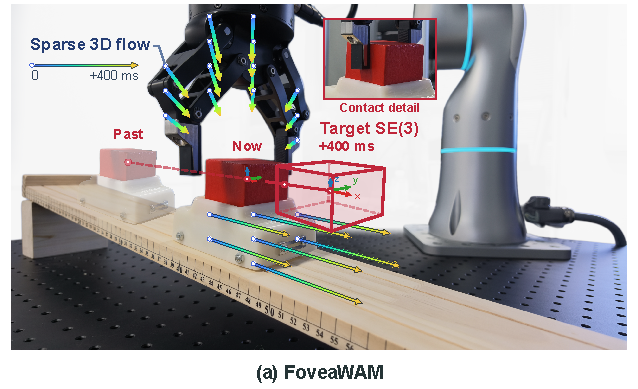
\includegraphics[width=.619178\textwidth]{figures/Fig1/real_scene.pdf}%
  \hfill
  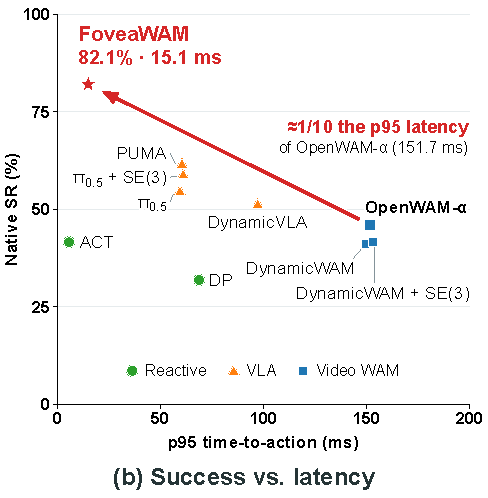
\includegraphics[width=.369863\textwidth]{figures/Fig1/native_tradeoff.pdf}%
}%
%
% \captionof{figure}{\textbf{\ours allocates prediction precision by role.}
% (a) It forecasts a precise SE(3) trajectory for the target and sparse 3D flow for its
% surroundings. (b) Success rate (SR) at native latency versus p95 time-to-action on \bench:
% \ours has the highest SR at about one tenth the latency of video world--action models.}
% \label{fig:teaser}
% \end{center}


% Official CVPR teaser pattern: the center environment adds the \topsep gap
% between the caption and the two-column body (a bare group adds none).
\begin{center}
\centering
\captionsetup{type=figure}
\resizebox{0.97\linewidth}{!}{%
    % Match the 2260:40:1350 widths of the previous 3650-unit canvas.
\makebox[\textwidth]{%
  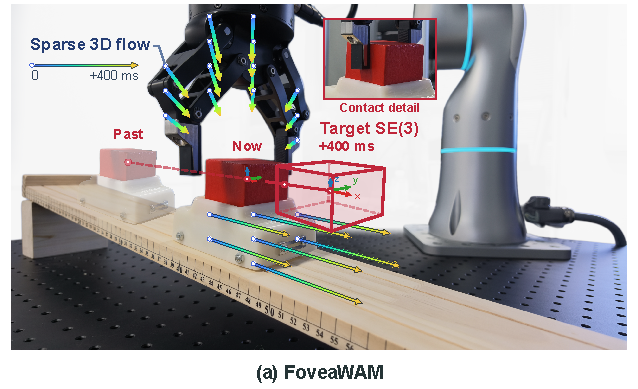
\includegraphics[width=.619178\textwidth]{figures/Fig1/real_scene.pdf}%
  \hfill
  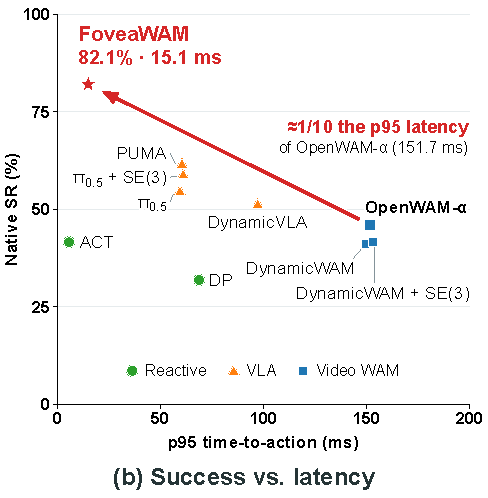
\includegraphics[width=.369863\textwidth]{figures/Fig1/native_tradeoff.pdf}%
}%
%
}\par
\captionof{figure}{\textbf{\ours allocates prediction precision by role.}
(a) Illustrative target SE(3) poses and sparse 3D flow. The inset shows a staged grasp.
(b) \ours leads in native SR on \bench at about one tenth the p95 latency of OpenWAM-$\alpha$.}
\label{fig:teaser}
\end{center}%